%%%%%%%%%%%%%%%%%%%%%%%%%%%%%%%%%%%%%%%%%%%%%%%%%%%%%%%%%%%%%%%

% Set up document

\documentclass{beamer}
\usecolortheme{whale}
\setbeamersize{text margin left=5mm,text margin right=5mm}

% Used to create a section slide between section
\AtBeginSection[]{
  \begin{frame}
  \vfill
  \centering
  \begin{beamercolorbox}[sep=8pt,center,shadow=true,rounded=true]{title}
    \usebeamerfont{title}\insertsectionhead\par%
  \end{beamercolorbox}
  \vfill
  \end{frame}
}

% Remove default navigation symbols and add just  page number
\setbeamertemplate{navigation symbols}{} % Clear default navigation
\addtobeamertemplate{navigation symbols}{}{%
    \usebeamerfont{footline}%
    \usebeamercolor[fg]{footline}%
    \hspace{1em}%
    \insertframenumber/\inserttotalframenumber
}

% CC licence
\usepackage[
    type={CC},
    modifier={by-nc-sa},
    version={3.0},
]{doclicense}

\usepackage{longtable}
%%%%%%%%%%%%%%%%%%%%%%%%%%%%%%%%%%%%%%%%%%%%%%%%%%%%%%%%%%%%%%%

% Title page

\title{What would other emergency stroke teams do?}
\subtitle{Using explainable machine learning to understand variation in thrombolysis practice}


\author{Kerry Pearn\inst{1}, Michael Allen\inst{1,3}, Anna Laws\inst{1}, Richard Everson\inst{3}, Martin James\inst{1,2} }
\institute{\inst{1}University of Exeter Medical School \inst{2}Royal Devon University Healthcare NHS Foundation Trust \inst{3}University of Exeter Institute of Data Science and Artificial Intelligence}

%\institute{Overleaf}
%\date{March 2023}


\begin{document}

%\frame{\titlepage}

\begin{frame}
\titlepage

\end{frame}


\begin{frame}
\frametitle{Sussex descriptive statistics (4hr arrivals)}

\scriptsize
\begin{table}[]
\begin{tabular}{llllll}
                            & All E+W & Worthing & St Richards & R. Sussex & Eastborn \\
\hline
thrombolysis (all arrivals)	        & 0.138	  & 0.167	 & 0.154	   & 0.106	   & 0.093    \\
onset known (all arrivals)          & 0.707   & 0.698    & 0.957       & 0.494     & 0.620    \\
arrive in 4 hours (all arrivals)    & 0.445   & 0.488    & 0.548       & 0.369     & 0.450    \\
\hline
age (approx*)                       & 75      & 79       & 79          & 77        & 79       \\
infarction                          & 0.849   & 0.842    & 0.824       & 0.834     & 0.860    \\
precise onset known                 & 0.637   & 0.453    & 0.522       & 0.742     & 0.751    \\
onset during sleep                  & 0.047   & 0.035    & 0.258       & 0.002     & 0.035    \\
use of AF anticoagulants            & 0.140   & 0.158    & 0.144       & 0.104     & 0.161    \\
prior disability                    & 1.114   & 1.498    & 1.708       & 1.311     & 1.206    \\
prestroke mrs 0-2	                & 0.785   &	0.735    & 0.660	   & 0.737     & 0.757    \\
stroke severity                     & 9.436   & 9.212    & 10.264      & 10.442    & 8.672    \\
onset-to-arrival time               & 102     & 94       & 107         & 95        & 99       \\
arrival-to-scan time                & 26      & 20       & 28          & 24        & 22       \\
thrombolysis                        & 0.303   & 0.335    & 0.280       & 0.276     & 0.200    \\
scan-to-thrombolysis time           & 30      & 35       & 29          & 31        & 40       \\
discharge disability                & 2.919   & 2.960    & 3.226       & 3.045     & 3.247    \\
death                               & 0.187   & 0.170    & 0.194       & 0.185     & 0.184    \\
increased mRS due to stroke         & 1.804   & 1.461    & 1.518       & 1.726     & 1.993    \\
mrs 5-6                             & 0.254   & 0.260    & 0.264       & 0.221     & 0.285    \\
mrs 0-2                             & 0.468   & 0.468    & 0.356       & 0.435     & 0.342   
\end{tabular}
\end{table}

\tiny
Out-of-hospital onset arrivals by ambulance. Main results block is for arrivals within 4 hours of known arrival by ambulance. Times are median times. All other values are means or proportions, as appropriate. *Age is based on 5 year age bands.

\end{frame}

\begin{frame}
\frametitle{Observed thrombolysis use in subgroups (1)}

  \begin{columns}[T]
    \begin{column}{0.5\textwidth}
      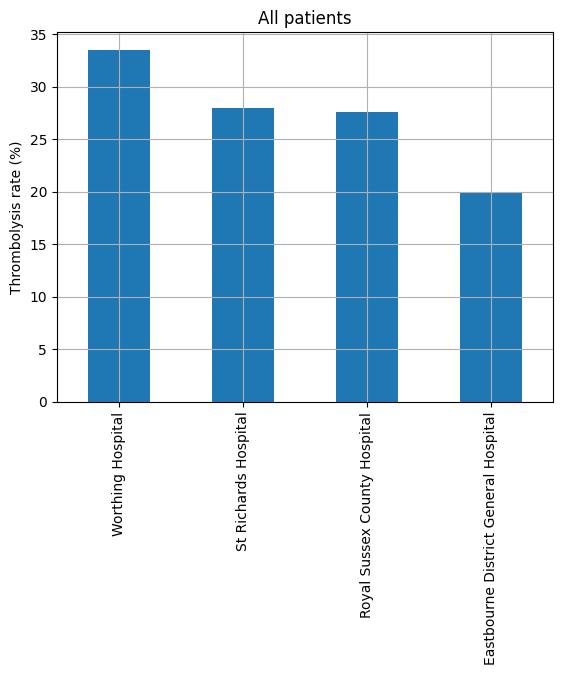
\includegraphics[width=1.0\textwidth]{./sussex/images/subgroup_all}
    \end{column}
    \begin{column}{0.5\textwidth}
      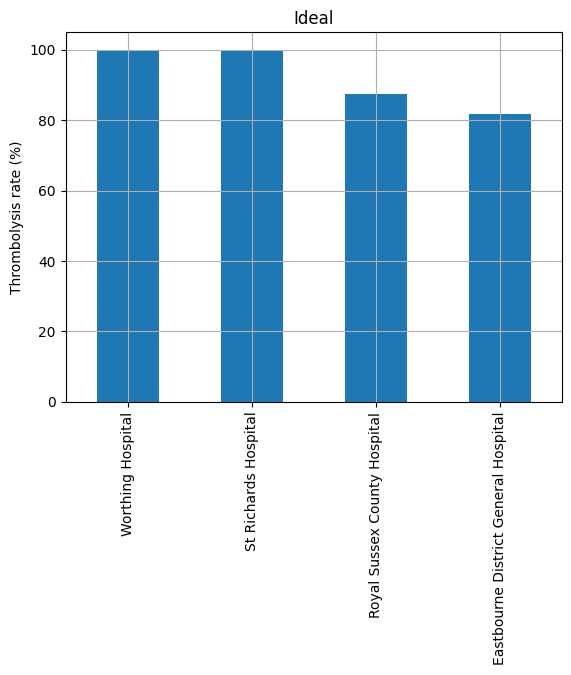
\includegraphics[width=1.0\textwidth]{./sussex/images/subgroup_ideal}
    \end{column}
  \end{columns}

\end{frame}

%%%%%%%%%%%%%%%%%%%%%%%%%%%%%%%%%%%%%%%%%%%%%%%%%%%%%%%%%%%%%%%%%%%%%%%%%%%%%%%%%

\begin{frame}
\frametitle{Observed thrombolysis use in subgroups (2)}

  \begin{columns}[T]
    \begin{column}{0.5\textwidth}
      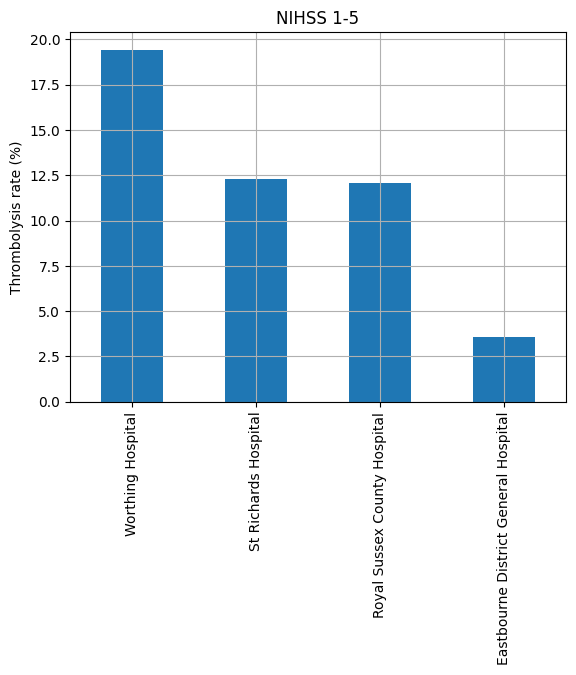
\includegraphics[width=1.0\textwidth]{./sussex/images/subgroup_mild}
    \end{column}
    \begin{column}{0.5\textwidth}
      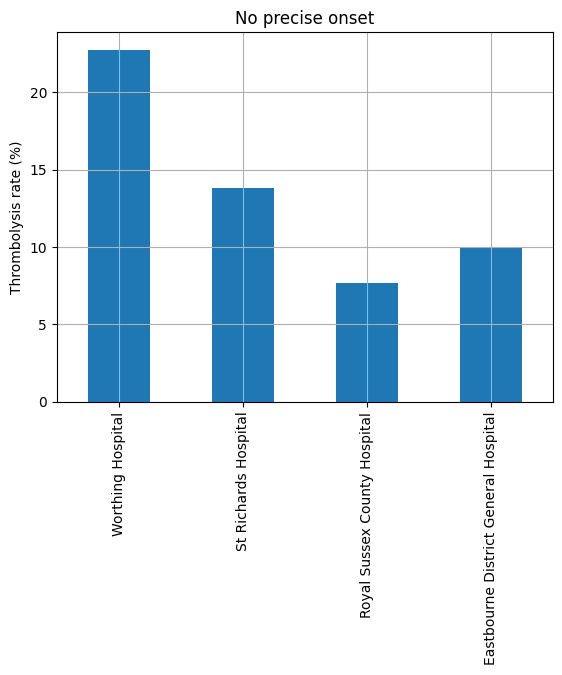
\includegraphics[width=1.0\textwidth]{./sussex/images/subgroup_precise}
    \end{column}
  \end{columns}

\end{frame}

%%%%%%%%%%%%%%%%%%%%%%%%%%%%%%%%%%%%%%%%%%%%%%%%%%%%%%%%%%%%%%%%%%%%%%%%%%%%%%%%%

\begin{frame}
\frametitle{Observed thrombolysis use in subgroups (3)}

  \begin{columns}[T]
    \begin{column}{0.5\textwidth}
      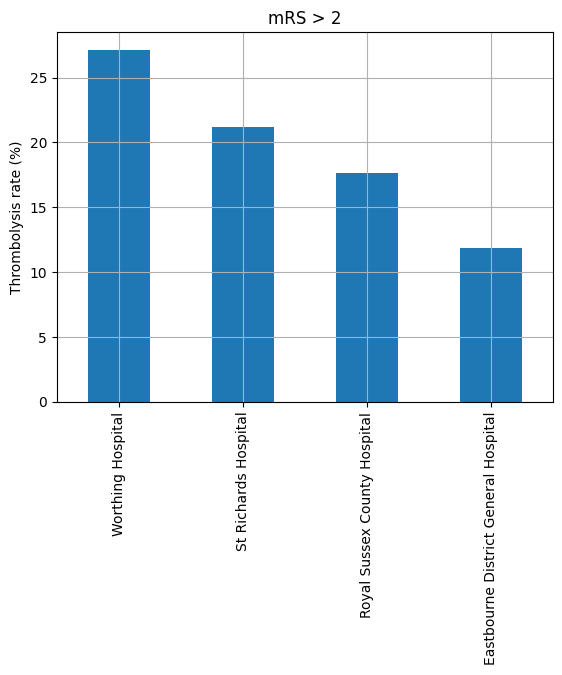
\includegraphics[width=1.0\textwidth]{./sussex/images/subgroup_disability}
    \end{column}
    \begin{column}{0.5\textwidth}
      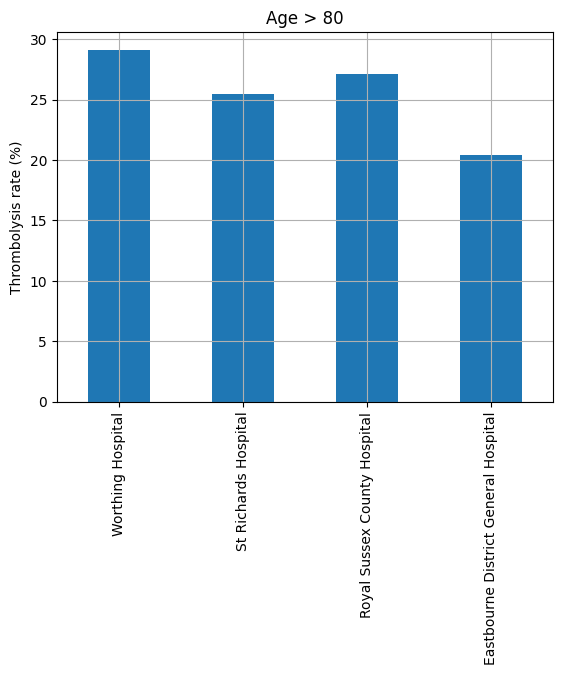
\includegraphics[width=1.0\textwidth]{./sussex/images/subgroup_age}
    \end{column}
  \end{columns}

\end{frame}






\begin{frame}
\frametitle{Benchmark thrombolysis decisions}


\begin{table}[]
\begin{tabular}{rrr}
                            & actual & benchmark \\
\hline
Worthing                    & 0.34   & 0.30      \\
St Richards                 & 0.28   & 0.29     \\
Royal Sussex County         & 0.28   & 0.43     \\
Eastbourne                  & 0.20   & 0.41
\end{tabular}
\end{table}

\end{frame}

%%%%%%%%%%%%%%%%%%%%%%%%%%%%%%%%%%%%%%%%%%%%%%%%%%%%%%%%%%%%%%%


\end{document}
